\documentclass[twoside]{book}

% Packages required by doxygen
\usepackage{fixltx2e}
\usepackage{calc}
\usepackage{doxygen}
\usepackage[export]{adjustbox} % also loads graphicx
\usepackage{graphicx}
\usepackage[utf8]{inputenc}
\usepackage{makeidx}
\usepackage{multicol}
\usepackage{multirow}
\PassOptionsToPackage{warn}{textcomp}
\usepackage{textcomp}
\usepackage[nointegrals]{wasysym}
\usepackage[table]{xcolor}

% Font selection
\usepackage[T1]{fontenc}
\usepackage[scaled=.90]{helvet}
\usepackage{courier}
\usepackage{amssymb}
\usepackage{sectsty}
\renewcommand{\familydefault}{\sfdefault}
\allsectionsfont{%
  \fontseries{bc}\selectfont%
  \color{darkgray}%
}
\renewcommand{\DoxyLabelFont}{%
  \fontseries{bc}\selectfont%
  \color{darkgray}%
}
\newcommand{\+}{\discretionary{\mbox{\scriptsize$\hookleftarrow$}}{}{}}

% Page & text layout
\usepackage{geometry}
\geometry{%
  a4paper,%
  top=2.5cm,%
  bottom=2.5cm,%
  left=2.5cm,%
  right=2.5cm%
}
\tolerance=750
\hfuzz=15pt
\hbadness=750
\setlength{\emergencystretch}{15pt}
\setlength{\parindent}{0cm}
\setlength{\parskip}{3ex plus 2ex minus 2ex}
\makeatletter
\renewcommand{\paragraph}{%
  \@startsection{paragraph}{4}{0ex}{-1.0ex}{1.0ex}{%
    \normalfont\normalsize\bfseries\SS@parafont%
  }%
}
\renewcommand{\subparagraph}{%
  \@startsection{subparagraph}{5}{0ex}{-1.0ex}{1.0ex}{%
    \normalfont\normalsize\bfseries\SS@subparafont%
  }%
}
\makeatother

% Headers & footers
\usepackage{fancyhdr}
\pagestyle{fancyplain}
\fancyhead[LE]{\fancyplain{}{\bfseries\thepage}}
\fancyhead[CE]{\fancyplain{}{}}
\fancyhead[RE]{\fancyplain{}{\bfseries\leftmark}}
\fancyhead[LO]{\fancyplain{}{\bfseries\rightmark}}
\fancyhead[CO]{\fancyplain{}{}}
\fancyhead[RO]{\fancyplain{}{\bfseries\thepage}}
\fancyfoot[LE]{\fancyplain{}{}}
\fancyfoot[CE]{\fancyplain{}{}}
\fancyfoot[RE]{\fancyplain{}{\bfseries\scriptsize Generated by Doxygen }}
\fancyfoot[LO]{\fancyplain{}{\bfseries\scriptsize Generated by Doxygen }}
\fancyfoot[CO]{\fancyplain{}{}}
\fancyfoot[RO]{\fancyplain{}{}}
\renewcommand{\footrulewidth}{0.4pt}
\renewcommand{\chaptermark}[1]{%
  \markboth{#1}{}%
}
\renewcommand{\sectionmark}[1]{%
  \markright{\thesection\ #1}%
}

% Indices & bibliography
\usepackage{natbib}
\usepackage[titles]{tocloft}
\setcounter{tocdepth}{3}
\setcounter{secnumdepth}{5}
\makeindex

% Hyperlinks (required, but should be loaded last)
\usepackage{ifpdf}
\ifpdf
  \usepackage[pdftex,pagebackref=true]{hyperref}
\else
  \usepackage[ps2pdf,pagebackref=true]{hyperref}
\fi
\hypersetup{%
  colorlinks=true,%
  linkcolor=blue,%
  citecolor=blue,%
  unicode%
}

% Custom commands
\newcommand{\clearemptydoublepage}{%
  \newpage{\pagestyle{empty}\cleardoublepage}%
}

\usepackage{caption}
\captionsetup{labelsep=space,justification=centering,font={bf},singlelinecheck=off,skip=4pt,position=top}

%===== C O N T E N T S =====

\begin{document}

% Titlepage & ToC
\hypersetup{pageanchor=false,
             bookmarksnumbered=true,
             pdfencoding=unicode
            }
\pagenumbering{alph}
\begin{titlepage}
\vspace*{7cm}
\begin{center}%
{\Large Cræft }\\
\vspace*{1cm}
{\large Generated by Doxygen 1.8.12}\\
\end{center}
\end{titlepage}
\clearemptydoublepage
\pagenumbering{roman}
\tableofcontents
\clearemptydoublepage
\pagenumbering{arabic}
\hypersetup{pageanchor=true}

%--- Begin generated contents ---
\chapter{Cr\&\#230;ft}
\label{md__r_e_a_d_m_e}
\hypertarget{md__r_e_a_d_m_e}{}
A new systems programming language, written for Caltech CS 81 with Donnie Pinkston as project mentor. 
\chapter{Module Index}
\section{Modules}
Here is a list of all modules\+:\begin{DoxyCompactList}
\item \contentsline{section}{Classes for possible types of tokens.}{\pageref{group___tokens}}{}
\begin{DoxyCompactList}
\item \contentsline{section}{Tokens with no meaning other than disambiguating syntax.}{\pageref{group___empty}}{}
\end{DoxyCompactList}
\end{DoxyCompactList}

\chapter{Hierarchical Index}
\section{Class Hierarchy}
This inheritance list is sorted roughly, but not completely, alphabetically\+:\begin{DoxyCompactList}
\item \contentsline{section}{Craeft\+:\+:A\+ST\+:\+:Binop}{\pageref{struct_craeft_1_1_a_s_t_1_1_binop}}{}
\item \contentsline{section}{Craeft\+:\+:A\+ST\+:\+:Cast}{\pageref{struct_craeft_1_1_a_s_t_1_1_cast}}{}
\item \contentsline{section}{Craeft\+:\+:Tok\+:\+:Close\+Brace}{\pageref{struct_craeft_1_1_tok_1_1_close_brace}}{}
\item \contentsline{section}{Craeft\+:\+:Tok\+:\+:Close\+Paren}{\pageref{struct_craeft_1_1_tok_1_1_close_paren}}{}
\item \contentsline{section}{Craeft\+:\+:Tok\+:\+:Comma}{\pageref{struct_craeft_1_1_tok_1_1_comma}}{}
\item \contentsline{section}{Craeft\+:\+:Double}{\pageref{struct_craeft_1_1_double}}{}
\item \contentsline{section}{Craeft\+:\+:Tok\+:\+:Else}{\pageref{struct_craeft_1_1_tok_1_1_else}}{}
\item \contentsline{section}{Craeft\+:\+:Float}{\pageref{struct_craeft_1_1_float}}{}
\item \contentsline{section}{Craeft\+:\+:Tok\+:\+:Float\+Literal}{\pageref{struct_craeft_1_1_tok_1_1_float_literal}}{}
\item \contentsline{section}{Craeft\+:\+:A\+ST\+:\+:Float\+Literal}{\pageref{struct_craeft_1_1_a_s_t_1_1_float_literal}}{}
\item \contentsline{section}{Craeft\+:\+:Tok\+:\+:Fn}{\pageref{struct_craeft_1_1_tok_1_1_fn}}{}
\item \contentsline{section}{Craeft\+:\+:A\+ST\+:\+:Function\+Call}{\pageref{struct_craeft_1_1_a_s_t_1_1_function_call}}{}
\item \contentsline{section}{Craeft\+:\+:Tok\+:\+:Identifier}{\pageref{struct_craeft_1_1_tok_1_1_identifier}}{}
\item \contentsline{section}{Craeft\+:\+:Tok\+:\+:If}{\pageref{struct_craeft_1_1_tok_1_1_if}}{}
\item \contentsline{section}{Craeft\+:\+:Tok\+:\+:Int\+Literal}{\pageref{struct_craeft_1_1_tok_1_1_int_literal}}{}
\item \contentsline{section}{Craeft\+:\+:A\+ST\+:\+:Int\+Literal}{\pageref{struct_craeft_1_1_a_s_t_1_1_int_literal}}{}
\item \contentsline{section}{Craeft\+:\+:Int\+Type}{\pageref{struct_craeft_1_1_int_type}}{}
\item \contentsline{section}{Craeft\+:\+:Lexer}{\pageref{class_craeft_1_1_lexer}}{}
\item \contentsline{section}{Craeft\+:\+:Tok\+:\+:Open\+Brace}{\pageref{struct_craeft_1_1_tok_1_1_open_brace}}{}
\item \contentsline{section}{Craeft\+:\+:Tok\+:\+:Open\+Paren}{\pageref{struct_craeft_1_1_tok_1_1_open_paren}}{}
\item \contentsline{section}{Craeft\+:\+:Tok\+:\+:Operator}{\pageref{struct_craeft_1_1_tok_1_1_operator}}{}
\item \contentsline{section}{Craeft\+:\+:Parser}{\pageref{class_craeft_1_1_parser}}{}
\item \contentsline{section}{Craeft\+:\+:Pointer}{\pageref{struct_craeft_1_1_pointer}}{}
\item \contentsline{section}{Craeft\+:\+:Tok\+:\+:Return}{\pageref{struct_craeft_1_1_tok_1_1_return}}{}
\item \contentsline{section}{Craeft\+:\+:Source\+Pos}{\pageref{struct_craeft_1_1_source_pos}}{}
\item static\+\_\+visitor\begin{DoxyCompactList}
\item \contentsline{section}{Craeft\+:\+:A\+ST\+:\+:Expression\+Print\+Visitor}{\pageref{struct_craeft_1_1_a_s_t_1_1_expression_print_visitor}}{}
\end{DoxyCompactList}
\item \contentsline{section}{Craeft\+:\+:Tok\+:\+:Struct}{\pageref{struct_craeft_1_1_tok_1_1_struct}}{}
\item \contentsline{section}{Craeft\+:\+:Tok\+:\+:Type\+Name}{\pageref{struct_craeft_1_1_tok_1_1_type_name}}{}
\item \contentsline{section}{Craeft\+:\+:A\+ST\+:\+:U\+Int\+Literal}{\pageref{struct_craeft_1_1_a_s_t_1_1_u_int_literal}}{}
\item \contentsline{section}{Craeft\+:\+:Tok\+:\+:U\+Int\+Literal}{\pageref{struct_craeft_1_1_tok_1_1_u_int_literal}}{}
\item \contentsline{section}{Craeft\+:\+:U\+Int\+Type}{\pageref{struct_craeft_1_1_u_int_type}}{}
\item \contentsline{section}{Craeft\+:\+:User\+Type}{\pageref{struct_craeft_1_1_user_type}}{}
\item \contentsline{section}{Craeft\+:\+:A\+ST\+:\+:Variable}{\pageref{struct_craeft_1_1_a_s_t_1_1_variable}}{}
\item \contentsline{section}{Craeft\+:\+:Tok\+:\+:While}{\pageref{struct_craeft_1_1_tok_1_1_while}}{}
\end{DoxyCompactList}

\chapter{Class Index}
\section{Class List}
Here are the classes, structs, unions and interfaces with brief descriptions\+:\begin{DoxyCompactList}
\item\contentsline{section}{\hyperlink{struct_craeft_1_1_a_s_t_1_1_binop}{Craeft\+::\+A\+S\+T\+::\+Binop} \\*Binary operator application }{\pageref{struct_craeft_1_1_a_s_t_1_1_binop}}{}
\item\contentsline{section}{\hyperlink{struct_craeft_1_1_a_s_t_1_1_cast}{Craeft\+::\+A\+S\+T\+::\+Cast} \\*Casts, from the syntactic form (Typename)expression }{\pageref{struct_craeft_1_1_a_s_t_1_1_cast}}{}
\item\contentsline{section}{\hyperlink{struct_craeft_1_1_tok_1_1_close_brace}{Craeft\+::\+Tok\+::\+Close\+Brace} }{\pageref{struct_craeft_1_1_tok_1_1_close_brace}}{}
\item\contentsline{section}{\hyperlink{struct_craeft_1_1_tok_1_1_close_paren}{Craeft\+::\+Tok\+::\+Close\+Paren} }{\pageref{struct_craeft_1_1_tok_1_1_close_paren}}{}
\item\contentsline{section}{\hyperlink{struct_craeft_1_1_tok_1_1_comma}{Craeft\+::\+Tok\+::\+Comma} }{\pageref{struct_craeft_1_1_tok_1_1_comma}}{}
\item\contentsline{section}{\hyperlink{struct_craeft_1_1_double}{Craeft\+::\+Double} \\*A double-\/precision float }{\pageref{struct_craeft_1_1_double}}{}
\item\contentsline{section}{\hyperlink{struct_craeft_1_1_tok_1_1_else}{Craeft\+::\+Tok\+::\+Else} }{\pageref{struct_craeft_1_1_tok_1_1_else}}{}
\item\contentsline{section}{\hyperlink{struct_craeft_1_1_a_s_t_1_1_expression_print_visitor}{Craeft\+::\+A\+S\+T\+::\+Expression\+Print\+Visitor} }{\pageref{struct_craeft_1_1_a_s_t_1_1_expression_print_visitor}}{}
\item\contentsline{section}{\hyperlink{struct_craeft_1_1_float}{Craeft\+::\+Float} \\*A single-\/precision float }{\pageref{struct_craeft_1_1_float}}{}
\item\contentsline{section}{\hyperlink{struct_craeft_1_1_tok_1_1_float_literal}{Craeft\+::\+Tok\+::\+Float\+Literal} \\*Floating-\/point literals }{\pageref{struct_craeft_1_1_tok_1_1_float_literal}}{}
\item\contentsline{section}{\hyperlink{struct_craeft_1_1_a_s_t_1_1_float_literal}{Craeft\+::\+A\+S\+T\+::\+Float\+Literal} \\*Floating-\/point literals }{\pageref{struct_craeft_1_1_a_s_t_1_1_float_literal}}{}
\item\contentsline{section}{\hyperlink{struct_craeft_1_1_tok_1_1_fn}{Craeft\+::\+Tok\+::\+Fn} }{\pageref{struct_craeft_1_1_tok_1_1_fn}}{}
\item\contentsline{section}{\hyperlink{struct_craeft_1_1_a_s_t_1_1_function_call}{Craeft\+::\+A\+S\+T\+::\+Function\+Call} \\*Function calls }{\pageref{struct_craeft_1_1_a_s_t_1_1_function_call}}{}
\item\contentsline{section}{\hyperlink{struct_craeft_1_1_tok_1_1_identifier}{Craeft\+::\+Tok\+::\+Identifier} \\*Non-\/type identifiers }{\pageref{struct_craeft_1_1_tok_1_1_identifier}}{}
\item\contentsline{section}{\hyperlink{struct_craeft_1_1_tok_1_1_if}{Craeft\+::\+Tok\+::\+If} }{\pageref{struct_craeft_1_1_tok_1_1_if}}{}
\item\contentsline{section}{\hyperlink{struct_craeft_1_1_tok_1_1_int_literal}{Craeft\+::\+Tok\+::\+Int\+Literal} \\*Signed integer literals }{\pageref{struct_craeft_1_1_tok_1_1_int_literal}}{}
\item\contentsline{section}{\hyperlink{struct_craeft_1_1_a_s_t_1_1_int_literal}{Craeft\+::\+A\+S\+T\+::\+Int\+Literal} \\*Signed integer literals }{\pageref{struct_craeft_1_1_a_s_t_1_1_int_literal}}{}
\item\contentsline{section}{\hyperlink{struct_craeft_1_1_int_type}{Craeft\+::\+Int\+Type} \\*A signed integer type }{\pageref{struct_craeft_1_1_int_type}}{}
\item\contentsline{section}{\hyperlink{class_craeft_1_1_lexer}{Craeft\+::\+Lexer} }{\pageref{class_craeft_1_1_lexer}}{}
\item\contentsline{section}{\hyperlink{struct_craeft_1_1_tok_1_1_open_brace}{Craeft\+::\+Tok\+::\+Open\+Brace} }{\pageref{struct_craeft_1_1_tok_1_1_open_brace}}{}
\item\contentsline{section}{\hyperlink{struct_craeft_1_1_tok_1_1_open_paren}{Craeft\+::\+Tok\+::\+Open\+Paren} }{\pageref{struct_craeft_1_1_tok_1_1_open_paren}}{}
\item\contentsline{section}{\hyperlink{struct_craeft_1_1_tok_1_1_operator}{Craeft\+::\+Tok\+::\+Operator} \\*Operators }{\pageref{struct_craeft_1_1_tok_1_1_operator}}{}
\item\contentsline{section}{\hyperlink{class_craeft_1_1_parser}{Craeft\+::\+Parser} }{\pageref{class_craeft_1_1_parser}}{}
\item\contentsline{section}{\hyperlink{struct_craeft_1_1_pointer}{Craeft\+::\+Pointer} \\*A pointer to another type }{\pageref{struct_craeft_1_1_pointer}}{}
\item\contentsline{section}{\hyperlink{struct_craeft_1_1_tok_1_1_return}{Craeft\+::\+Tok\+::\+Return} }{\pageref{struct_craeft_1_1_tok_1_1_return}}{}
\item\contentsline{section}{\hyperlink{struct_craeft_1_1_source_pos}{Craeft\+::\+Source\+Pos} }{\pageref{struct_craeft_1_1_source_pos}}{}
\item\contentsline{section}{\hyperlink{struct_craeft_1_1_tok_1_1_struct}{Craeft\+::\+Tok\+::\+Struct} }{\pageref{struct_craeft_1_1_tok_1_1_struct}}{}
\item\contentsline{section}{\hyperlink{struct_craeft_1_1_tok_1_1_type_name}{Craeft\+::\+Tok\+::\+Type\+Name} \\*Names of types }{\pageref{struct_craeft_1_1_tok_1_1_type_name}}{}
\item\contentsline{section}{\hyperlink{struct_craeft_1_1_a_s_t_1_1_u_int_literal}{Craeft\+::\+A\+S\+T\+::\+U\+Int\+Literal} \\*Unsigned integer literals }{\pageref{struct_craeft_1_1_a_s_t_1_1_u_int_literal}}{}
\item\contentsline{section}{\hyperlink{struct_craeft_1_1_tok_1_1_u_int_literal}{Craeft\+::\+Tok\+::\+U\+Int\+Literal} \\*Unsigned integer literals }{\pageref{struct_craeft_1_1_tok_1_1_u_int_literal}}{}
\item\contentsline{section}{\hyperlink{struct_craeft_1_1_u_int_type}{Craeft\+::\+U\+Int\+Type} \\*An unsigned integer type }{\pageref{struct_craeft_1_1_u_int_type}}{}
\item\contentsline{section}{\hyperlink{struct_craeft_1_1_user_type}{Craeft\+::\+User\+Type} \\*Any other type }{\pageref{struct_craeft_1_1_user_type}}{}
\item\contentsline{section}{\hyperlink{struct_craeft_1_1_a_s_t_1_1_variable}{Craeft\+::\+A\+S\+T\+::\+Variable} \\*Variables }{\pageref{struct_craeft_1_1_a_s_t_1_1_variable}}{}
\item\contentsline{section}{\hyperlink{struct_craeft_1_1_tok_1_1_while}{Craeft\+::\+Tok\+::\+While} }{\pageref{struct_craeft_1_1_tok_1_1_while}}{}
\end{DoxyCompactList}

\chapter{File Index}
\section{File List}
Here is a list of all documented files with brief descriptions\+:\begin{DoxyCompactList}
\item\contentsline{section}{{\bfseries .\+ycm\+\_\+extra\+\_\+conf\+\_\+c++.\+py} }{\pageref{_8ycm__extra__conf__c_09_09_8py}}{}
\item\contentsline{section}{\hyperlink{_error_8hh}{Error.\+hh} \\*Error handling and related utilities }{\pageref{_error_8hh}}{}
\item\contentsline{section}{\hyperlink{expr__parse__demo_8cpp}{expr\+\_\+parse\+\_\+demo.\+cpp} }{\pageref{expr__parse__demo_8cpp}}{}
\item\contentsline{section}{\hyperlink{_expression_8cpp}{Expression.\+cpp} }{\pageref{_expression_8cpp}}{}
\item\contentsline{section}{\hyperlink{_expression_8hh}{Expression.\+hh} \\*The classes comprising the expression portion of the A\+ST }{\pageref{_expression_8hh}}{}
\item\contentsline{section}{\hyperlink{_lexer_8cpp}{Lexer.\+cpp} }{\pageref{_lexer_8cpp}}{}
\item\contentsline{section}{{\bfseries Lexer.\+hh} }{\pageref{_lexer_8hh}}{}
\item\contentsline{section}{\hyperlink{_parser_8cpp}{Parser.\+cpp} }{\pageref{_parser_8cpp}}{}
\item\contentsline{section}{\hyperlink{_parser_8hh}{Parser.\+hh} \\*The parser }{\pageref{_parser_8hh}}{}
\item\contentsline{section}{\hyperlink{_token_8hh}{Token.\+hh} \\*Tokens as output by the lexer }{\pageref{_token_8hh}}{}
\item\contentsline{section}{\hyperlink{_type_8hh}{Type.\+hh} \\*Types as represented in the compiler }{\pageref{_type_8hh}}{}
\item\contentsline{section}{\hyperlink{_variant_utils_8hh}{Variant\+Utils.\+hh} }{\pageref{_variant_utils_8hh}}{}
\end{DoxyCompactList}

\chapter{Module Documentation}
\hypertarget{group___tokens}{}\section{Classes for possible types of tokens.}
\label{group___tokens}\index{Classes for possible types of tokens.@{Classes for possible types of tokens.}}
\subsection*{Modules}
\begin{DoxyCompactItemize}
\item 
\hyperlink{group___empty}{Tokens with no meaning other than disambiguating syntax.}
\end{DoxyCompactItemize}
\subsection*{Classes}
\begin{DoxyCompactItemize}
\item 
struct \hyperlink{struct_craeft_1_1_tok_1_1_type_name}{Craeft\+::\+Tok\+::\+Type\+Name}
\begin{DoxyCompactList}\small\item\em Names of types. \end{DoxyCompactList}\item 
struct \hyperlink{struct_craeft_1_1_tok_1_1_identifier}{Craeft\+::\+Tok\+::\+Identifier}
\begin{DoxyCompactList}\small\item\em Non-\/type identifiers. \end{DoxyCompactList}\item 
struct \hyperlink{struct_craeft_1_1_tok_1_1_int_literal}{Craeft\+::\+Tok\+::\+Int\+Literal}
\begin{DoxyCompactList}\small\item\em Signed integer literals. \end{DoxyCompactList}\item 
struct \hyperlink{struct_craeft_1_1_tok_1_1_u_int_literal}{Craeft\+::\+Tok\+::\+U\+Int\+Literal}
\begin{DoxyCompactList}\small\item\em Unsigned integer literals. \end{DoxyCompactList}\item 
struct \hyperlink{struct_craeft_1_1_tok_1_1_float_literal}{Craeft\+::\+Tok\+::\+Float\+Literal}
\begin{DoxyCompactList}\small\item\em Floating-\/point literals. \end{DoxyCompactList}\item 
struct \hyperlink{struct_craeft_1_1_tok_1_1_operator}{Craeft\+::\+Tok\+::\+Operator}
\begin{DoxyCompactList}\small\item\em Operators. \end{DoxyCompactList}\item 
struct \hyperlink{struct_craeft_1_1_tok_1_1_open_paren}{Craeft\+::\+Tok\+::\+Open\+Paren}
\item 
struct \hyperlink{struct_craeft_1_1_tok_1_1_close_paren}{Craeft\+::\+Tok\+::\+Close\+Paren}
\item 
struct \hyperlink{struct_craeft_1_1_tok_1_1_open_brace}{Craeft\+::\+Tok\+::\+Open\+Brace}
\item 
struct \hyperlink{struct_craeft_1_1_tok_1_1_close_brace}{Craeft\+::\+Tok\+::\+Close\+Brace}
\item 
struct \hyperlink{struct_craeft_1_1_tok_1_1_comma}{Craeft\+::\+Tok\+::\+Comma}
\item 
struct \hyperlink{struct_craeft_1_1_tok_1_1_fn}{Craeft\+::\+Tok\+::\+Fn}
\item 
struct \hyperlink{struct_craeft_1_1_tok_1_1_struct}{Craeft\+::\+Tok\+::\+Struct}
\item 
struct \hyperlink{struct_craeft_1_1_tok_1_1_return}{Craeft\+::\+Tok\+::\+Return}
\item 
struct \hyperlink{struct_craeft_1_1_tok_1_1_if}{Craeft\+::\+Tok\+::\+If}
\item 
struct \hyperlink{struct_craeft_1_1_tok_1_1_else}{Craeft\+::\+Tok\+::\+Else}
\item 
struct \hyperlink{struct_craeft_1_1_tok_1_1_while}{Craeft\+::\+Tok\+::\+While}
\end{DoxyCompactItemize}


\subsection{Detailed Description}
Each of these classes contains public data members for the contents of the token and a simple inline constructor which takes one argument per member. For performance, these constructors will {\ttfamily move} potentially expensive-\/to-\/copy data like strings. 
\hypertarget{group___empty}{}\section{Tokens with no meaning other than disambiguating syntax.}
\label{group___empty}\index{Tokens with no meaning other than disambiguating syntax.@{Tokens with no meaning other than disambiguating syntax.}}

\chapter{Class Documentation}
\hypertarget{struct_craeft_1_1_a_s_t_1_1_binop}{}\section{Craeft\+:\+:A\+ST\+:\+:Binop Struct Reference}
\label{struct_craeft_1_1_a_s_t_1_1_binop}\index{Craeft\+::\+A\+S\+T\+::\+Binop@{Craeft\+::\+A\+S\+T\+::\+Binop}}


Binary operator application.  




{\ttfamily \#include $<$Expression.\+hh$>$}

\subsection*{Public Member Functions}
\begin{DoxyCompactItemize}
\item 
\hypertarget{struct_craeft_1_1_a_s_t_1_1_binop_ac5de457f8ffa1b7e049636ca1766444f}{}\label{struct_craeft_1_1_a_s_t_1_1_binop_ac5de457f8ffa1b7e049636ca1766444f} 
{\bfseries Binop} (std\+::string op, \hyperlink{_expression_8hh_aef28cabf6d8e7cb8324232e27e69606d}{Expression} lhs, \hyperlink{_expression_8hh_aef28cabf6d8e7cb8324232e27e69606d}{Expression} rhs, \hyperlink{struct_craeft_1_1_source_pos}{Source\+Pos} pos)
\end{DoxyCompactItemize}
\subsection*{Public Attributes}
\begin{DoxyCompactItemize}
\item 
\hypertarget{struct_craeft_1_1_a_s_t_1_1_binop_a84a57322d7117fcf8f7cd308db30a58e}{}\label{struct_craeft_1_1_a_s_t_1_1_binop_a84a57322d7117fcf8f7cd308db30a58e} 
std\+::string {\bfseries op}
\item 
\hypertarget{struct_craeft_1_1_a_s_t_1_1_binop_ae6942fdd35f86322bbeef3071a85fd7c}{}\label{struct_craeft_1_1_a_s_t_1_1_binop_ae6942fdd35f86322bbeef3071a85fd7c} 
\hyperlink{_expression_8hh_aef28cabf6d8e7cb8324232e27e69606d}{Expression} {\bfseries lhs}
\item 
\hypertarget{struct_craeft_1_1_a_s_t_1_1_binop_a958de46985886bfe01f5459938b247f0}{}\label{struct_craeft_1_1_a_s_t_1_1_binop_a958de46985886bfe01f5459938b247f0} 
\hyperlink{_expression_8hh_aef28cabf6d8e7cb8324232e27e69606d}{Expression} {\bfseries rhs}
\item 
\hypertarget{struct_craeft_1_1_a_s_t_1_1_binop_aed1d3282f356adbefa8bd0273340b7f2}{}\label{struct_craeft_1_1_a_s_t_1_1_binop_aed1d3282f356adbefa8bd0273340b7f2} 
\hyperlink{struct_craeft_1_1_source_pos}{Source\+Pos} {\bfseries pos}
\end{DoxyCompactItemize}


\subsection{Detailed Description}
Binary operator application. 

Definition at line 104 of file Expression.\+hh.



The documentation for this struct was generated from the following file\+:\begin{DoxyCompactItemize}
\item 
\hyperlink{_expression_8hh}{Expression.\+hh}\end{DoxyCompactItemize}

\hypertarget{struct_craeft_1_1_a_s_t_1_1_cast}{}\section{Craeft\+:\+:A\+ST\+:\+:Cast Struct Reference}
\label{struct_craeft_1_1_a_s_t_1_1_cast}\index{Craeft\+::\+A\+S\+T\+::\+Cast@{Craeft\+::\+A\+S\+T\+::\+Cast}}


Casts, from the syntactic form (Typename)expression.  




{\ttfamily \#include $<$Expression.\+hh$>$}

\subsection*{Public Member Functions}
\begin{DoxyCompactItemize}
\item 
\hypertarget{struct_craeft_1_1_a_s_t_1_1_cast_ab79620730fc07cc380283f7e6e604386}{}\label{struct_craeft_1_1_a_s_t_1_1_cast_ab79620730fc07cc380283f7e6e604386} 
{\bfseries Cast} (std\+::unique\+\_\+ptr$<$ Type $>$ t, \hyperlink{_expression_8hh_aef28cabf6d8e7cb8324232e27e69606d}{Expression} arg, \hyperlink{struct_craeft_1_1_source_pos}{Source\+Pos} pos)
\end{DoxyCompactItemize}
\subsection*{Public Attributes}
\begin{DoxyCompactItemize}
\item 
\hypertarget{struct_craeft_1_1_a_s_t_1_1_cast_a82df15337155e1d0aeec6c41196977fd}{}\label{struct_craeft_1_1_a_s_t_1_1_cast_a82df15337155e1d0aeec6c41196977fd} 
std\+::unique\+\_\+ptr$<$ Type $>$ {\bfseries t}
\item 
\hypertarget{struct_craeft_1_1_a_s_t_1_1_cast_a64862fda4902db196344900dc2ac7a07}{}\label{struct_craeft_1_1_a_s_t_1_1_cast_a64862fda4902db196344900dc2ac7a07} 
\hyperlink{_expression_8hh_aef28cabf6d8e7cb8324232e27e69606d}{Expression} {\bfseries arg}
\item 
\hypertarget{struct_craeft_1_1_a_s_t_1_1_cast_a16f9f448dcd013ae9b4c7dc68f64029b}{}\label{struct_craeft_1_1_a_s_t_1_1_cast_a16f9f448dcd013ae9b4c7dc68f64029b} 
\hyperlink{struct_craeft_1_1_source_pos}{Source\+Pos} {\bfseries pos}
\end{DoxyCompactItemize}


\subsection{Detailed Description}
Casts, from the syntactic form (Typename)expression. 

Definition at line 137 of file Expression.\+hh.



The documentation for this struct was generated from the following file\+:\begin{DoxyCompactItemize}
\item 
\hyperlink{_expression_8hh}{Expression.\+hh}\end{DoxyCompactItemize}

\hypertarget{struct_craeft_1_1_tok_1_1_close_brace}{}\section{Craeft\+:\+:Tok\+:\+:Close\+Brace Struct Reference}
\label{struct_craeft_1_1_tok_1_1_close_brace}\index{Craeft\+::\+Tok\+::\+Close\+Brace@{Craeft\+::\+Tok\+::\+Close\+Brace}}


\subsection{Detailed Description}


Definition at line 111 of file Token.\+hh.



The documentation for this struct was generated from the following file\+:\begin{DoxyCompactItemize}
\item 
\hyperlink{_token_8hh}{Token.\+hh}\end{DoxyCompactItemize}

\hypertarget{struct_craeft_1_1_tok_1_1_close_paren}{}\section{Craeft\+:\+:Tok\+:\+:Close\+Paren Struct Reference}
\label{struct_craeft_1_1_tok_1_1_close_paren}\index{Craeft\+::\+Tok\+::\+Close\+Paren@{Craeft\+::\+Tok\+::\+Close\+Paren}}


\subsection{Detailed Description}


Definition at line 109 of file Token.\+hh.



The documentation for this struct was generated from the following file\+:\begin{DoxyCompactItemize}
\item 
\hyperlink{_token_8hh}{Token.\+hh}\end{DoxyCompactItemize}

\hypertarget{struct_craeft_1_1_tok_1_1_comma}{}\section{Craeft\+:\+:Tok\+:\+:Comma Struct Reference}
\label{struct_craeft_1_1_tok_1_1_comma}\index{Craeft\+::\+Tok\+::\+Comma@{Craeft\+::\+Tok\+::\+Comma}}


\subsection{Detailed Description}


Definition at line 112 of file Token.\+hh.



The documentation for this struct was generated from the following file\+:\begin{DoxyCompactItemize}
\item 
\hyperlink{_token_8hh}{Token.\+hh}\end{DoxyCompactItemize}

\hypertarget{struct_craeft_1_1_double}{}\section{Craeft\+:\+:Double Struct Reference}
\label{struct_craeft_1_1_double}\index{Craeft\+::\+Double@{Craeft\+::\+Double}}


A double-\/precision float.  




{\ttfamily \#include $<$Type.\+hh$>$}



\subsection{Detailed Description}
A double-\/precision float. 

Definition at line 61 of file Type.\+hh.



The documentation for this struct was generated from the following file\+:\begin{DoxyCompactItemize}
\item 
\hyperlink{_type_8hh}{Type.\+hh}\end{DoxyCompactItemize}

\hypertarget{struct_craeft_1_1_tok_1_1_else}{}\section{Craeft\+:\+:Tok\+:\+:Else Struct Reference}
\label{struct_craeft_1_1_tok_1_1_else}\index{Craeft\+::\+Tok\+::\+Else@{Craeft\+::\+Tok\+::\+Else}}


\subsection{Detailed Description}


Definition at line 117 of file Token.\+hh.



The documentation for this struct was generated from the following file\+:\begin{DoxyCompactItemize}
\item 
\hyperlink{_token_8hh}{Token.\+hh}\end{DoxyCompactItemize}

\hypertarget{struct_craeft_1_1_a_s_t_1_1_expression_print_visitor}{}\section{Craeft\+:\+:A\+ST\+:\+:Expression\+Print\+Visitor Struct Reference}
\label{struct_craeft_1_1_a_s_t_1_1_expression_print_visitor}\index{Craeft\+::\+A\+S\+T\+::\+Expression\+Print\+Visitor@{Craeft\+::\+A\+S\+T\+::\+Expression\+Print\+Visitor}}
Inheritance diagram for Craeft\+:\+:A\+ST\+:\+:Expression\+Print\+Visitor\+:\begin{figure}[H]
\begin{center}
\leavevmode
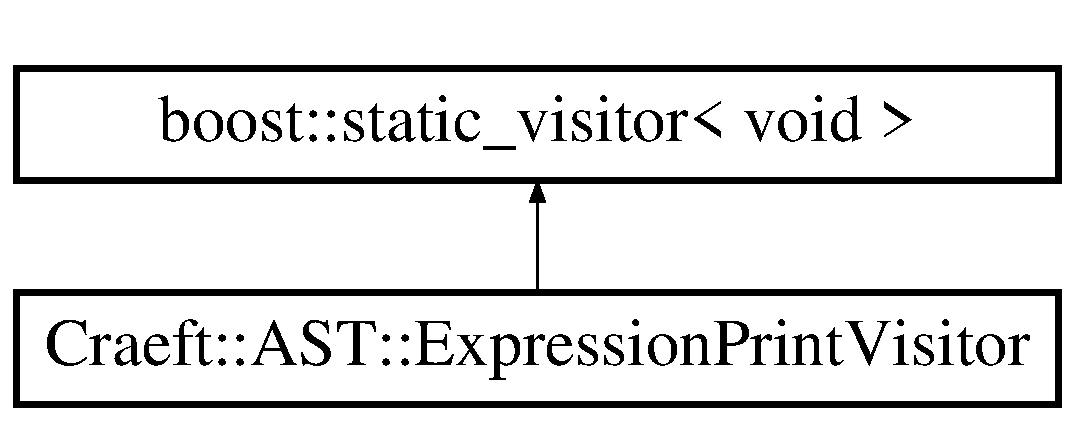
\includegraphics[height=2.000000cm]{struct_craeft_1_1_a_s_t_1_1_expression_print_visitor}
\end{center}
\end{figure}
\subsection*{Public Member Functions}
\begin{DoxyCompactItemize}
\item 
\hypertarget{struct_craeft_1_1_a_s_t_1_1_expression_print_visitor_a4748b28753ef931037b4c9b3e34c0055}{}\label{struct_craeft_1_1_a_s_t_1_1_expression_print_visitor_a4748b28753ef931037b4c9b3e34c0055} 
{\bfseries Expression\+Print\+Visitor} (std\+::ostream \&out)
\item 
\hypertarget{struct_craeft_1_1_a_s_t_1_1_expression_print_visitor_acbd09f31d916d91ba63dc952cf4722ba}{}\label{struct_craeft_1_1_a_s_t_1_1_expression_print_visitor_acbd09f31d916d91ba63dc952cf4722ba} 
{\footnotesize template$<$typename T $>$ }\\void {\bfseries operator()} (const T \&lit)
\item 
\hypertarget{struct_craeft_1_1_a_s_t_1_1_expression_print_visitor_aeb2d0eb54931d3f73037083de8cafbe4}{}\label{struct_craeft_1_1_a_s_t_1_1_expression_print_visitor_aeb2d0eb54931d3f73037083de8cafbe4} 
void {\bfseries operator()} (const \hyperlink{struct_craeft_1_1_a_s_t_1_1_variable}{Variable} \&var)
\item 
\hypertarget{struct_craeft_1_1_a_s_t_1_1_expression_print_visitor_a8dc5fecbb36ab796a8a5aafea15f9df2}{}\label{struct_craeft_1_1_a_s_t_1_1_expression_print_visitor_a8dc5fecbb36ab796a8a5aafea15f9df2} 
void {\bfseries operator()} (const std\+::unique\+\_\+ptr$<$ \hyperlink{struct_craeft_1_1_a_s_t_1_1_binop}{Binop} $>$ \&bin)
\item 
\hypertarget{struct_craeft_1_1_a_s_t_1_1_expression_print_visitor_abaaf0952418ae731e17df5267d413e73}{}\label{struct_craeft_1_1_a_s_t_1_1_expression_print_visitor_abaaf0952418ae731e17df5267d413e73} 
void {\bfseries operator()} (const std\+::unique\+\_\+ptr$<$ \hyperlink{struct_craeft_1_1_a_s_t_1_1_function_call}{Function\+Call} $>$ \&fc)
\item 
\hypertarget{struct_craeft_1_1_a_s_t_1_1_expression_print_visitor_affc09118165703f172b92b7a5c33355c}{}\label{struct_craeft_1_1_a_s_t_1_1_expression_print_visitor_affc09118165703f172b92b7a5c33355c} 
void {\bfseries operator()} (const std\+::unique\+\_\+ptr$<$ \hyperlink{struct_craeft_1_1_a_s_t_1_1_cast}{Cast} $>$ \&c)
\end{DoxyCompactItemize}
\subsection*{Public Attributes}
\begin{DoxyCompactItemize}
\item 
\hypertarget{struct_craeft_1_1_a_s_t_1_1_expression_print_visitor_a604b7caef0b71da99a6d8eb3a58a3957}{}\label{struct_craeft_1_1_a_s_t_1_1_expression_print_visitor_a604b7caef0b71da99a6d8eb3a58a3957} 
std\+::ostream \& {\bfseries out}
\end{DoxyCompactItemize}


\subsection{Detailed Description}


Definition at line 31 of file Expression.\+cpp.



The documentation for this struct was generated from the following file\+:\begin{DoxyCompactItemize}
\item 
\hyperlink{_expression_8cpp}{Expression.\+cpp}\end{DoxyCompactItemize}

\hypertarget{struct_craeft_1_1_float}{}\section{Craeft\+:\+:Float Struct Reference}
\label{struct_craeft_1_1_float}\index{Craeft\+::\+Float@{Craeft\+::\+Float}}


A single-\/precision float.  




{\ttfamily \#include $<$Type.\+hh$>$}



\subsection{Detailed Description}
A single-\/precision float. 

Definition at line 56 of file Type.\+hh.



The documentation for this struct was generated from the following file\+:\begin{DoxyCompactItemize}
\item 
\hyperlink{_type_8hh}{Type.\+hh}\end{DoxyCompactItemize}

\hypertarget{struct_craeft_1_1_tok_1_1_float_literal}{}\section{Craeft\+:\+:Tok\+:\+:Float\+Literal Struct Reference}
\label{struct_craeft_1_1_tok_1_1_float_literal}\index{Craeft\+::\+Tok\+::\+Float\+Literal@{Craeft\+::\+Tok\+::\+Float\+Literal}}


Floating-\/point literals.  




{\ttfamily \#include $<$Token.\+hh$>$}

\subsection*{Public Member Functions}
\begin{DoxyCompactItemize}
\item 
\hypertarget{struct_craeft_1_1_tok_1_1_float_literal_ab2c97907c6014737f47c8a08929c3ca6}{}\label{struct_craeft_1_1_tok_1_1_float_literal_ab2c97907c6014737f47c8a08929c3ca6} 
{\bfseries Float\+Literal} (double value)
\end{DoxyCompactItemize}
\subsection*{Public Attributes}
\begin{DoxyCompactItemize}
\item 
\hypertarget{struct_craeft_1_1_tok_1_1_float_literal_a702ffc031f709726368dbbda18df9e92}{}\label{struct_craeft_1_1_tok_1_1_float_literal_a702ffc031f709726368dbbda18df9e92} 
double {\bfseries value}
\end{DoxyCompactItemize}


\subsection{Detailed Description}
Floating-\/point literals. 

Definition at line 89 of file Token.\+hh.



The documentation for this struct was generated from the following file\+:\begin{DoxyCompactItemize}
\item 
\hyperlink{_token_8hh}{Token.\+hh}\end{DoxyCompactItemize}

\hypertarget{struct_craeft_1_1_a_s_t_1_1_float_literal}{}\section{Craeft\+:\+:A\+ST\+:\+:Float\+Literal Struct Reference}
\label{struct_craeft_1_1_a_s_t_1_1_float_literal}\index{Craeft\+::\+A\+S\+T\+::\+Float\+Literal@{Craeft\+::\+A\+S\+T\+::\+Float\+Literal}}


Floating-\/point literals.  




{\ttfamily \#include $<$Expression.\+hh$>$}

\subsection*{Public Member Functions}
\begin{DoxyCompactItemize}
\item 
\hypertarget{struct_craeft_1_1_a_s_t_1_1_float_literal_a2148f616f0df8fa9e9f947efc0ea6480}{}\label{struct_craeft_1_1_a_s_t_1_1_float_literal_a2148f616f0df8fa9e9f947efc0ea6480} 
{\bfseries Float\+Literal} (double value, \hyperlink{struct_craeft_1_1_source_pos}{Source\+Pos} pos)
\end{DoxyCompactItemize}
\subsection*{Public Attributes}
\begin{DoxyCompactItemize}
\item 
\hypertarget{struct_craeft_1_1_a_s_t_1_1_float_literal_abfdc3f38d5f64c213ad507d55fee550d}{}\label{struct_craeft_1_1_a_s_t_1_1_float_literal_abfdc3f38d5f64c213ad507d55fee550d} 
double {\bfseries value}
\item 
\hypertarget{struct_craeft_1_1_a_s_t_1_1_float_literal_a221cba0856d46d03f6da874e4a79f679}{}\label{struct_craeft_1_1_a_s_t_1_1_float_literal_a221cba0856d46d03f6da874e4a79f679} 
\hyperlink{struct_craeft_1_1_source_pos}{Source\+Pos} {\bfseries pos}
\end{DoxyCompactItemize}


\subsection{Detailed Description}
Floating-\/point literals. 

Definition at line 66 of file Expression.\+hh.



The documentation for this struct was generated from the following file\+:\begin{DoxyCompactItemize}
\item 
\hyperlink{_expression_8hh}{Expression.\+hh}\end{DoxyCompactItemize}

\hypertarget{struct_craeft_1_1_tok_1_1_fn}{}\section{Craeft\+:\+:Tok\+:\+:Fn Struct Reference}
\label{struct_craeft_1_1_tok_1_1_fn}\index{Craeft\+::\+Tok\+::\+Fn@{Craeft\+::\+Tok\+::\+Fn}}


\subsection{Detailed Description}


Definition at line 113 of file Token.\+hh.



The documentation for this struct was generated from the following file\+:\begin{DoxyCompactItemize}
\item 
\hyperlink{_token_8hh}{Token.\+hh}\end{DoxyCompactItemize}

\hypertarget{struct_craeft_1_1_a_s_t_1_1_function_call}{}\section{Craeft\+:\+:A\+ST\+:\+:Function\+Call Struct Reference}
\label{struct_craeft_1_1_a_s_t_1_1_function_call}\index{Craeft\+::\+A\+S\+T\+::\+Function\+Call@{Craeft\+::\+A\+S\+T\+::\+Function\+Call}}


Function calls.  




{\ttfamily \#include $<$Expression.\+hh$>$}

\subsection*{Public Member Functions}
\begin{DoxyCompactItemize}
\item 
\hypertarget{struct_craeft_1_1_a_s_t_1_1_function_call_a58f4f65e86b7ae1162132d9bdfc7cda4}{}\label{struct_craeft_1_1_a_s_t_1_1_function_call_a58f4f65e86b7ae1162132d9bdfc7cda4} 
{\bfseries Function\+Call} (std\+::string fname, std\+::vector$<$ \hyperlink{_expression_8hh_aef28cabf6d8e7cb8324232e27e69606d}{Expression} $>$ args, \hyperlink{struct_craeft_1_1_source_pos}{Source\+Pos} pos)
\end{DoxyCompactItemize}
\subsection*{Public Attributes}
\begin{DoxyCompactItemize}
\item 
\hypertarget{struct_craeft_1_1_a_s_t_1_1_function_call_aeec640c9e76dcf9535fcebc5ceb86417}{}\label{struct_craeft_1_1_a_s_t_1_1_function_call_aeec640c9e76dcf9535fcebc5ceb86417} 
std\+::string {\bfseries fname}
\item 
\hypertarget{struct_craeft_1_1_a_s_t_1_1_function_call_a4f96ccf063fdb97b846ed84381bb6357}{}\label{struct_craeft_1_1_a_s_t_1_1_function_call_a4f96ccf063fdb97b846ed84381bb6357} 
std\+::vector$<$ \hyperlink{_expression_8hh_aef28cabf6d8e7cb8324232e27e69606d}{Expression} $>$ {\bfseries args}
\item 
\hypertarget{struct_craeft_1_1_a_s_t_1_1_function_call_a1f4d2de6af42eb28db5a2a9557155afb}{}\label{struct_craeft_1_1_a_s_t_1_1_function_call_a1f4d2de6af42eb28db5a2a9557155afb} 
\hyperlink{struct_craeft_1_1_source_pos}{Source\+Pos} {\bfseries pos}
\end{DoxyCompactItemize}


\subsection{Detailed Description}
Function calls. 

Definition at line 121 of file Expression.\+hh.



The documentation for this struct was generated from the following file\+:\begin{DoxyCompactItemize}
\item 
\hyperlink{_expression_8hh}{Expression.\+hh}\end{DoxyCompactItemize}

\hypertarget{struct_craeft_1_1_tok_1_1_identifier}{}\section{Craeft\+:\+:Tok\+:\+:Identifier Struct Reference}
\label{struct_craeft_1_1_tok_1_1_identifier}\index{Craeft\+::\+Tok\+::\+Identifier@{Craeft\+::\+Tok\+::\+Identifier}}


Non-\/type identifiers.  




{\ttfamily \#include $<$Token.\+hh$>$}

\subsection*{Public Member Functions}
\begin{DoxyCompactItemize}
\item 
\hypertarget{struct_craeft_1_1_tok_1_1_identifier_acdc709d34c4a75c47d25292d14b92db6}{}\label{struct_craeft_1_1_tok_1_1_identifier_acdc709d34c4a75c47d25292d14b92db6} 
{\bfseries Identifier} (std\+::string name)
\end{DoxyCompactItemize}
\subsection*{Public Attributes}
\begin{DoxyCompactItemize}
\item 
\hypertarget{struct_craeft_1_1_tok_1_1_identifier_a6ff35ba5863ea7e8b0510a47cee73594}{}\label{struct_craeft_1_1_tok_1_1_identifier_a6ff35ba5863ea7e8b0510a47cee73594} 
std\+::string {\bfseries name}
\end{DoxyCompactItemize}


\subsection{Detailed Description}
Non-\/type identifiers. 

Definition at line 62 of file Token.\+hh.



The documentation for this struct was generated from the following file\+:\begin{DoxyCompactItemize}
\item 
\hyperlink{_token_8hh}{Token.\+hh}\end{DoxyCompactItemize}

\hypertarget{struct_craeft_1_1_tok_1_1_if}{}\section{Craeft\+:\+:Tok\+:\+:If Struct Reference}
\label{struct_craeft_1_1_tok_1_1_if}\index{Craeft\+::\+Tok\+::\+If@{Craeft\+::\+Tok\+::\+If}}


\subsection{Detailed Description}


Definition at line 116 of file Token.\+hh.



The documentation for this struct was generated from the following file\+:\begin{DoxyCompactItemize}
\item 
\hyperlink{_token_8hh}{Token.\+hh}\end{DoxyCompactItemize}

\hypertarget{struct_craeft_1_1_tok_1_1_int_literal}{}\section{Craeft\+:\+:Tok\+:\+:Int\+Literal Struct Reference}
\label{struct_craeft_1_1_tok_1_1_int_literal}\index{Craeft\+::\+Tok\+::\+Int\+Literal@{Craeft\+::\+Tok\+::\+Int\+Literal}}


Signed integer literals.  




{\ttfamily \#include $<$Token.\+hh$>$}

\subsection*{Public Member Functions}
\begin{DoxyCompactItemize}
\item 
\hypertarget{struct_craeft_1_1_tok_1_1_int_literal_a0ea408d10dabcb273e10a0b48a9bbf63}{}\label{struct_craeft_1_1_tok_1_1_int_literal_a0ea408d10dabcb273e10a0b48a9bbf63} 
{\bfseries Int\+Literal} (int64\+\_\+t value)
\end{DoxyCompactItemize}
\subsection*{Public Attributes}
\begin{DoxyCompactItemize}
\item 
\hypertarget{struct_craeft_1_1_tok_1_1_int_literal_ab113edf4246f583fba2cc0f1551cb5a0}{}\label{struct_craeft_1_1_tok_1_1_int_literal_ab113edf4246f583fba2cc0f1551cb5a0} 
int64\+\_\+t {\bfseries value}
\end{DoxyCompactItemize}


\subsection{Detailed Description}
Signed integer literals. 

Definition at line 71 of file Token.\+hh.



The documentation for this struct was generated from the following file\+:\begin{DoxyCompactItemize}
\item 
\hyperlink{_token_8hh}{Token.\+hh}\end{DoxyCompactItemize}

\hypertarget{struct_craeft_1_1_a_s_t_1_1_int_literal}{}\section{Craeft\+:\+:A\+ST\+:\+:Int\+Literal Struct Reference}
\label{struct_craeft_1_1_a_s_t_1_1_int_literal}\index{Craeft\+::\+A\+S\+T\+::\+Int\+Literal@{Craeft\+::\+A\+S\+T\+::\+Int\+Literal}}


Signed integer literals.  




{\ttfamily \#include $<$Expression.\+hh$>$}

\subsection*{Public Member Functions}
\begin{DoxyCompactItemize}
\item 
\hypertarget{struct_craeft_1_1_a_s_t_1_1_int_literal_a094cc3c63b8b5762312fe0720801c4de}{}\label{struct_craeft_1_1_a_s_t_1_1_int_literal_a094cc3c63b8b5762312fe0720801c4de} 
{\bfseries Int\+Literal} (int64\+\_\+t value, \hyperlink{struct_craeft_1_1_source_pos}{Source\+Pos} pos)
\end{DoxyCompactItemize}
\subsection*{Public Attributes}
\begin{DoxyCompactItemize}
\item 
\hypertarget{struct_craeft_1_1_a_s_t_1_1_int_literal_a18d15284860c74ab021c55a498c7bb46}{}\label{struct_craeft_1_1_a_s_t_1_1_int_literal_a18d15284860c74ab021c55a498c7bb46} 
int64\+\_\+t {\bfseries value}
\item 
\hypertarget{struct_craeft_1_1_a_s_t_1_1_int_literal_a350599f201b1277802d2c2d77e39562e}{}\label{struct_craeft_1_1_a_s_t_1_1_int_literal_a350599f201b1277802d2c2d77e39562e} 
\hyperlink{struct_craeft_1_1_source_pos}{Source\+Pos} {\bfseries pos}
\end{DoxyCompactItemize}


\subsection{Detailed Description}
Signed integer literals. 

Definition at line 46 of file Expression.\+hh.



The documentation for this struct was generated from the following file\+:\begin{DoxyCompactItemize}
\item 
\hyperlink{_expression_8hh}{Expression.\+hh}\end{DoxyCompactItemize}

\hypertarget{struct_craeft_1_1_int_type}{}\section{Craeft\+:\+:Int\+Type Struct Reference}
\label{struct_craeft_1_1_int_type}\index{Craeft\+::\+Int\+Type@{Craeft\+::\+Int\+Type}}


A signed integer type.  




{\ttfamily \#include $<$Type.\+hh$>$}

\subsection*{Public Member Functions}
\begin{DoxyCompactItemize}
\item 
\hypertarget{struct_craeft_1_1_int_type_aa878af97376f5d00b53be1c339cb5075}{}\label{struct_craeft_1_1_int_type_aa878af97376f5d00b53be1c339cb5075} 
{\bfseries Int\+Type} (int nbits)
\end{DoxyCompactItemize}
\subsection*{Public Attributes}
\begin{DoxyCompactItemize}
\item 
\hypertarget{struct_craeft_1_1_int_type_a49597f2ccedcd46664615192e897e6a5}{}\label{struct_craeft_1_1_int_type_a49597f2ccedcd46664615192e897e6a5} 
int {\bfseries nbits}
\end{DoxyCompactItemize}


\subsection{Detailed Description}
A signed integer type. 

Definition at line 38 of file Type.\+hh.



The documentation for this struct was generated from the following file\+:\begin{DoxyCompactItemize}
\item 
\hyperlink{_type_8hh}{Type.\+hh}\end{DoxyCompactItemize}

\hypertarget{class_craeft_1_1_lexer}{}\section{Craeft\+:\+:Lexer Class Reference}
\label{class_craeft_1_1_lexer}\index{Craeft\+::\+Lexer@{Craeft\+::\+Lexer}}
\subsection*{Public Member Functions}
\begin{DoxyCompactItemize}
\item 
\hyperlink{class_craeft_1_1_lexer_a52dbd45faef58e7ea838d02cd7198037}{Lexer} (std\+::string fname)
\begin{DoxyCompactList}\small\item\em Create a new lexer, tokenizing the given input stream. \end{DoxyCompactList}\item 
\hypertarget{class_craeft_1_1_lexer_ae63a7e1707391ab861ed9195a2b1cca6}{}\label{class_craeft_1_1_lexer_ae63a7e1707391ab861ed9195a2b1cca6} 
\hyperlink{struct_craeft_1_1_source_pos}{Source\+Pos} \hyperlink{class_craeft_1_1_lexer_ae63a7e1707391ab861ed9195a2b1cca6}{get\+\_\+pos} (void) const
\begin{DoxyCompactList}\small\item\em Get the position the lexer is currently at. \end{DoxyCompactList}\item 
\hypertarget{class_craeft_1_1_lexer_a92ce6b920fff270ac55c9542207c0d4d}{}\label{class_craeft_1_1_lexer_a92ce6b920fff270ac55c9542207c0d4d} 
\hyperlink{_token_8hh_a521c5743a63e2d5d1871557794e0a8b1}{Tok\+::\+Token} \hyperlink{class_craeft_1_1_lexer_a92ce6b920fff270ac55c9542207c0d4d}{get\+\_\+tok} (void) const
\begin{DoxyCompactList}\small\item\em Return the last lexed token. \end{DoxyCompactList}\item 
\hypertarget{class_craeft_1_1_lexer_ac3b24e7a7f9202ab54550334904dd008}{}\label{class_craeft_1_1_lexer_ac3b24e7a7f9202ab54550334904dd008} 
bool \hyperlink{class_craeft_1_1_lexer_ac3b24e7a7f9202ab54550334904dd008}{at\+\_\+eof} () const
\begin{DoxyCompactList}\small\item\em Return whether the lexer has reached the end of the stream. \end{DoxyCompactList}\item 
\hypertarget{class_craeft_1_1_lexer_a64a72871a0d35c35d07e887fd39d0d70}{}\label{class_craeft_1_1_lexer_a64a72871a0d35c35d07e887fd39d0d70} 
void \hyperlink{class_craeft_1_1_lexer_a64a72871a0d35c35d07e887fd39d0d70}{shift} (void)
\begin{DoxyCompactList}\small\item\em Lex a new token. \end{DoxyCompactList}\end{DoxyCompactItemize}


\subsection{Detailed Description}


Definition at line 40 of file Lexer.\+hh.



\subsection{Constructor \& Destructor Documentation}
\hypertarget{class_craeft_1_1_lexer_a52dbd45faef58e7ea838d02cd7198037}{}\label{class_craeft_1_1_lexer_a52dbd45faef58e7ea838d02cd7198037} 
\index{Craeft\+::\+Lexer@{Craeft\+::\+Lexer}!Lexer@{Lexer}}
\index{Lexer@{Lexer}!Craeft\+::\+Lexer@{Craeft\+::\+Lexer}}
\subsubsection{\texorpdfstring{Lexer()}{Lexer()}}
{\footnotesize\ttfamily Craeft\+::\+Lexer\+::\+Lexer (\begin{DoxyParamCaption}\item[{std\+::string}]{fname }\end{DoxyParamCaption})}



Create a new lexer, tokenizing the given input stream. 


\begin{DoxyParams}{Parameters}
{\em fname} & The name of the file to tokenize. \\
\hline
\end{DoxyParams}


Definition at line 30 of file Lexer.\+cpp.



The documentation for this class was generated from the following files\+:\begin{DoxyCompactItemize}
\item 
Lexer.\+hh\item 
\hyperlink{_lexer_8cpp}{Lexer.\+cpp}\end{DoxyCompactItemize}

\hypertarget{struct_craeft_1_1_tok_1_1_open_brace}{}\section{Craeft\+:\+:Tok\+:\+:Open\+Brace Struct Reference}
\label{struct_craeft_1_1_tok_1_1_open_brace}\index{Craeft\+::\+Tok\+::\+Open\+Brace@{Craeft\+::\+Tok\+::\+Open\+Brace}}


\subsection{Detailed Description}


Definition at line 110 of file Token.\+hh.



The documentation for this struct was generated from the following file\+:\begin{DoxyCompactItemize}
\item 
\hyperlink{_token_8hh}{Token.\+hh}\end{DoxyCompactItemize}

\hypertarget{struct_craeft_1_1_tok_1_1_open_paren}{}\section{Craeft\+:\+:Tok\+:\+:Open\+Paren Struct Reference}
\label{struct_craeft_1_1_tok_1_1_open_paren}\index{Craeft\+::\+Tok\+::\+Open\+Paren@{Craeft\+::\+Tok\+::\+Open\+Paren}}


\subsection{Detailed Description}


Definition at line 108 of file Token.\+hh.



The documentation for this struct was generated from the following file\+:\begin{DoxyCompactItemize}
\item 
\hyperlink{_token_8hh}{Token.\+hh}\end{DoxyCompactItemize}

\hypertarget{struct_craeft_1_1_tok_1_1_operator}{}\section{Craeft\+:\+:Tok\+:\+:Operator Struct Reference}
\label{struct_craeft_1_1_tok_1_1_operator}\index{Craeft\+::\+Tok\+::\+Operator@{Craeft\+::\+Tok\+::\+Operator}}


Operators.  




{\ttfamily \#include $<$Token.\+hh$>$}

\subsection*{Public Member Functions}
\begin{DoxyCompactItemize}
\item 
\hypertarget{struct_craeft_1_1_tok_1_1_operator_a181a1f4d3d94cc46cd69e95ee0a827cb}{}\label{struct_craeft_1_1_tok_1_1_operator_a181a1f4d3d94cc46cd69e95ee0a827cb} 
{\bfseries Operator} (std\+::string op)
\end{DoxyCompactItemize}
\subsection*{Public Attributes}
\begin{DoxyCompactItemize}
\item 
\hypertarget{struct_craeft_1_1_tok_1_1_operator_aba2aae639d4decca354ae44999e8907c}{}\label{struct_craeft_1_1_tok_1_1_operator_aba2aae639d4decca354ae44999e8907c} 
std\+::string {\bfseries op}
\end{DoxyCompactItemize}


\subsection{Detailed Description}
Operators. 

Definition at line 98 of file Token.\+hh.



The documentation for this struct was generated from the following file\+:\begin{DoxyCompactItemize}
\item 
\hyperlink{_token_8hh}{Token.\+hh}\end{DoxyCompactItemize}

\hypertarget{class_craeft_1_1_parser}{}\section{Craeft\+:\+:Parser Class Reference}
\label{class_craeft_1_1_parser}\index{Craeft\+::\+Parser@{Craeft\+::\+Parser}}
\subsection*{Public Member Functions}
\begin{DoxyCompactItemize}
\item 
\hyperlink{class_craeft_1_1_parser_a584edbe348c503996ad4f0583b843520}{Parser} (std\+::string fname)
\begin{DoxyCompactList}\small\item\em Create a new \hyperlink{class_craeft_1_1_parser}{Parser}, parsing from the given file. \end{DoxyCompactList}\item 
\hyperlink{_expression_8hh_aef28cabf6d8e7cb8324232e27e69606d}{A\+S\+T\+::\+Expression} \hyperlink{class_craeft_1_1_parser_ae991d774fc82c09ec4a4223b883580a9}{parse\+\_\+expression} (void)
\begin{DoxyCompactList}\small\item\em Parse the next expression from the lexer. \end{DoxyCompactList}\end{DoxyCompactItemize}


\subsection{Detailed Description}


Definition at line 34 of file Parser.\+hh.



\subsection{Constructor \& Destructor Documentation}
\hypertarget{class_craeft_1_1_parser_a584edbe348c503996ad4f0583b843520}{}\label{class_craeft_1_1_parser_a584edbe348c503996ad4f0583b843520} 
\index{Craeft\+::\+Parser@{Craeft\+::\+Parser}!Parser@{Parser}}
\index{Parser@{Parser}!Craeft\+::\+Parser@{Craeft\+::\+Parser}}
\subsubsection{\texorpdfstring{Parser()}{Parser()}}
{\footnotesize\ttfamily Craeft\+::\+Parser\+::\+Parser (\begin{DoxyParamCaption}\item[{std\+::string}]{fname }\end{DoxyParamCaption})}



Create a new \hyperlink{class_craeft_1_1_parser}{Parser}, parsing from the given file. 


\begin{DoxyParams}{Parameters}
{\em fname} & The filename to open and parse from. \\
\hline
\end{DoxyParams}


Definition at line 42 of file Parser.\+cpp.



\subsection{Member Function Documentation}
\hypertarget{class_craeft_1_1_parser_ae991d774fc82c09ec4a4223b883580a9}{}\label{class_craeft_1_1_parser_ae991d774fc82c09ec4a4223b883580a9} 
\index{Craeft\+::\+Parser@{Craeft\+::\+Parser}!parse\+\_\+expression@{parse\+\_\+expression}}
\index{parse\+\_\+expression@{parse\+\_\+expression}!Craeft\+::\+Parser@{Craeft\+::\+Parser}}
\subsubsection{\texorpdfstring{parse\+\_\+expression()}{parse\_expression()}}
{\footnotesize\ttfamily \hyperlink{_expression_8hh_aef28cabf6d8e7cb8324232e27e69606d}{A\+S\+T\+::\+Expression} Craeft\+::\+Parser\+::parse\+\_\+expression (\begin{DoxyParamCaption}\item[{void}]{ }\end{DoxyParamCaption})}



Parse the next expression from the lexer. 

Start at the token the lexer is {\itshape currently} on. 

Definition at line 44 of file Parser.\+cpp.



The documentation for this class was generated from the following files\+:\begin{DoxyCompactItemize}
\item 
\hyperlink{_parser_8hh}{Parser.\+hh}\item 
\hyperlink{_parser_8cpp}{Parser.\+cpp}\end{DoxyCompactItemize}

\hypertarget{struct_craeft_1_1_pointer}{}\section{Craeft\+:\+:Pointer Struct Reference}
\label{struct_craeft_1_1_pointer}\index{Craeft\+::\+Pointer@{Craeft\+::\+Pointer}}


A pointer to another type.  




{\ttfamily \#include $<$Type.\+hh$>$}

\subsection*{Public Attributes}
\begin{DoxyCompactItemize}
\item 
\hypertarget{struct_craeft_1_1_pointer_a3bd9b25e171f9fa66a7ddf06e533b025}{}\label{struct_craeft_1_1_pointer_a3bd9b25e171f9fa66a7ddf06e533b025} 
Type {\bfseries pointed}
\end{DoxyCompactItemize}


\subsection{Detailed Description}
A pointer to another type. 

Definition at line 80 of file Type.\+hh.



The documentation for this struct was generated from the following file\+:\begin{DoxyCompactItemize}
\item 
\hyperlink{_type_8hh}{Type.\+hh}\end{DoxyCompactItemize}

\hypertarget{struct_craeft_1_1_tok_1_1_return}{}\section{Craeft\+:\+:Tok\+:\+:Return Struct Reference}
\label{struct_craeft_1_1_tok_1_1_return}\index{Craeft\+::\+Tok\+::\+Return@{Craeft\+::\+Tok\+::\+Return}}


\subsection{Detailed Description}


Definition at line 115 of file Token.\+hh.



The documentation for this struct was generated from the following file\+:\begin{DoxyCompactItemize}
\item 
\hyperlink{_token_8hh}{Token.\+hh}\end{DoxyCompactItemize}

\hypertarget{struct_craeft_1_1_source_pos}{}\section{Craeft\+:\+:Source\+Pos Struct Reference}
\label{struct_craeft_1_1_source_pos}\index{Craeft\+::\+Source\+Pos@{Craeft\+::\+Source\+Pos}}
\subsection*{Public Member Functions}
\begin{DoxyCompactItemize}
\item 
\hypertarget{struct_craeft_1_1_source_pos_a8bdad625b6772cbc447aaa470a6182de}{}\label{struct_craeft_1_1_source_pos_a8bdad625b6772cbc447aaa470a6182de} 
{\bfseries Source\+Pos} (uint16\+\_\+t charno, uint16\+\_\+t lineno)
\end{DoxyCompactItemize}
\subsection*{Public Attributes}
\begin{DoxyCompactItemize}
\item 
\hypertarget{struct_craeft_1_1_source_pos_a8158cf29de6026a22439dd55864c822e}{}\label{struct_craeft_1_1_source_pos_a8158cf29de6026a22439dd55864c822e} 
uint16\+\_\+t {\bfseries charno}
\item 
\hypertarget{struct_craeft_1_1_source_pos_aacb508675e6f3373c3e80593c21f79f6}{}\label{struct_craeft_1_1_source_pos_aacb508675e6f3373c3e80593c21f79f6} 
uint16\+\_\+t {\bfseries lineno}
\end{DoxyCompactItemize}


\subsection{Detailed Description}


Definition at line 31 of file Error.\+hh.



The documentation for this struct was generated from the following file\+:\begin{DoxyCompactItemize}
\item 
\hyperlink{_error_8hh}{Error.\+hh}\end{DoxyCompactItemize}

\hypertarget{struct_craeft_1_1_tok_1_1_struct}{}\section{Craeft\+:\+:Tok\+:\+:Struct Struct Reference}
\label{struct_craeft_1_1_tok_1_1_struct}\index{Craeft\+::\+Tok\+::\+Struct@{Craeft\+::\+Tok\+::\+Struct}}


\subsection{Detailed Description}


Definition at line 114 of file Token.\+hh.



The documentation for this struct was generated from the following file\+:\begin{DoxyCompactItemize}
\item 
\hyperlink{_token_8hh}{Token.\+hh}\end{DoxyCompactItemize}

\hypertarget{struct_craeft_1_1_tok_1_1_type_name}{}\section{Craeft\+:\+:Tok\+:\+:Type\+Name Struct Reference}
\label{struct_craeft_1_1_tok_1_1_type_name}\index{Craeft\+::\+Tok\+::\+Type\+Name@{Craeft\+::\+Tok\+::\+Type\+Name}}


Names of types.  




{\ttfamily \#include $<$Token.\+hh$>$}

\subsection*{Public Member Functions}
\begin{DoxyCompactItemize}
\item 
\hypertarget{struct_craeft_1_1_tok_1_1_type_name_adf5fcea8e780d71f3a79de97da40e4a9}{}\label{struct_craeft_1_1_tok_1_1_type_name_adf5fcea8e780d71f3a79de97da40e4a9} 
{\bfseries Type\+Name} (std\+::string name)
\end{DoxyCompactItemize}
\subsection*{Public Attributes}
\begin{DoxyCompactItemize}
\item 
\hypertarget{struct_craeft_1_1_tok_1_1_type_name_a868758b94e212af6ae44bcd819c23ef7}{}\label{struct_craeft_1_1_tok_1_1_type_name_a868758b94e212af6ae44bcd819c23ef7} 
std\+::string {\bfseries name}
\end{DoxyCompactItemize}


\subsection{Detailed Description}
Names of types. 

Definition at line 53 of file Token.\+hh.



The documentation for this struct was generated from the following file\+:\begin{DoxyCompactItemize}
\item 
\hyperlink{_token_8hh}{Token.\+hh}\end{DoxyCompactItemize}

\hypertarget{struct_craeft_1_1_a_s_t_1_1_u_int_literal}{}\section{Craeft\+:\+:A\+ST\+:\+:U\+Int\+Literal Struct Reference}
\label{struct_craeft_1_1_a_s_t_1_1_u_int_literal}\index{Craeft\+::\+A\+S\+T\+::\+U\+Int\+Literal@{Craeft\+::\+A\+S\+T\+::\+U\+Int\+Literal}}


Unsigned integer literals.  




{\ttfamily \#include $<$Expression.\+hh$>$}

\subsection*{Public Member Functions}
\begin{DoxyCompactItemize}
\item 
\hypertarget{struct_craeft_1_1_a_s_t_1_1_u_int_literal_a0ba04a1f2d84bd7b25292a0d5f4c6bd8}{}\label{struct_craeft_1_1_a_s_t_1_1_u_int_literal_a0ba04a1f2d84bd7b25292a0d5f4c6bd8} 
{\bfseries U\+Int\+Literal} (uint64\+\_\+t value, \hyperlink{struct_craeft_1_1_source_pos}{Source\+Pos} pos)
\end{DoxyCompactItemize}
\subsection*{Public Attributes}
\begin{DoxyCompactItemize}
\item 
\hypertarget{struct_craeft_1_1_a_s_t_1_1_u_int_literal_a3dec720d3171bca88cc94f03b53e9d35}{}\label{struct_craeft_1_1_a_s_t_1_1_u_int_literal_a3dec720d3171bca88cc94f03b53e9d35} 
uint64\+\_\+t {\bfseries value}
\item 
\hypertarget{struct_craeft_1_1_a_s_t_1_1_u_int_literal_ac4a1cf0179981a33d2278918ea5ff155}{}\label{struct_craeft_1_1_a_s_t_1_1_u_int_literal_ac4a1cf0179981a33d2278918ea5ff155} 
\hyperlink{struct_craeft_1_1_source_pos}{Source\+Pos} {\bfseries pos}
\end{DoxyCompactItemize}


\subsection{Detailed Description}
Unsigned integer literals. 

Definition at line 56 of file Expression.\+hh.



The documentation for this struct was generated from the following file\+:\begin{DoxyCompactItemize}
\item 
\hyperlink{_expression_8hh}{Expression.\+hh}\end{DoxyCompactItemize}

\hypertarget{struct_craeft_1_1_tok_1_1_u_int_literal}{}\section{Craeft\+:\+:Tok\+:\+:U\+Int\+Literal Struct Reference}
\label{struct_craeft_1_1_tok_1_1_u_int_literal}\index{Craeft\+::\+Tok\+::\+U\+Int\+Literal@{Craeft\+::\+Tok\+::\+U\+Int\+Literal}}


Unsigned integer literals.  




{\ttfamily \#include $<$Token.\+hh$>$}

\subsection*{Public Member Functions}
\begin{DoxyCompactItemize}
\item 
\hypertarget{struct_craeft_1_1_tok_1_1_u_int_literal_ac7c51c66686b37c38bbf9f533097ab1e}{}\label{struct_craeft_1_1_tok_1_1_u_int_literal_ac7c51c66686b37c38bbf9f533097ab1e} 
{\bfseries U\+Int\+Literal} (uint64\+\_\+t value)
\end{DoxyCompactItemize}
\subsection*{Public Attributes}
\begin{DoxyCompactItemize}
\item 
\hypertarget{struct_craeft_1_1_tok_1_1_u_int_literal_a4322d36bd8c9e997d73ecc71a91adbc3}{}\label{struct_craeft_1_1_tok_1_1_u_int_literal_a4322d36bd8c9e997d73ecc71a91adbc3} 
uint64\+\_\+t {\bfseries value}
\end{DoxyCompactItemize}


\subsection{Detailed Description}
Unsigned integer literals. 

Definition at line 80 of file Token.\+hh.



The documentation for this struct was generated from the following file\+:\begin{DoxyCompactItemize}
\item 
\hyperlink{_token_8hh}{Token.\+hh}\end{DoxyCompactItemize}

\hypertarget{struct_craeft_1_1_u_int_type}{}\section{Craeft\+:\+:U\+Int\+Type Struct Reference}
\label{struct_craeft_1_1_u_int_type}\index{Craeft\+::\+U\+Int\+Type@{Craeft\+::\+U\+Int\+Type}}


An unsigned integer type.  




{\ttfamily \#include $<$Type.\+hh$>$}

\subsection*{Public Member Functions}
\begin{DoxyCompactItemize}
\item 
\hypertarget{struct_craeft_1_1_u_int_type_a9e7db452453f5649ed76a0ca6898181d}{}\label{struct_craeft_1_1_u_int_type_a9e7db452453f5649ed76a0ca6898181d} 
{\bfseries U\+Int\+Type} (int nbits)
\end{DoxyCompactItemize}
\subsection*{Public Attributes}
\begin{DoxyCompactItemize}
\item 
\hypertarget{struct_craeft_1_1_u_int_type_aa7a8e31c6d8daf58e8894a9abea60599}{}\label{struct_craeft_1_1_u_int_type_aa7a8e31c6d8daf58e8894a9abea60599} 
int {\bfseries nbits}
\end{DoxyCompactItemize}


\subsection{Detailed Description}
An unsigned integer type. 

Definition at line 47 of file Type.\+hh.



The documentation for this struct was generated from the following file\+:\begin{DoxyCompactItemize}
\item 
\hyperlink{_type_8hh}{Type.\+hh}\end{DoxyCompactItemize}

\hypertarget{struct_craeft_1_1_user_type}{}\section{Craeft\+:\+:User\+Type Struct Reference}
\label{struct_craeft_1_1_user_type}\index{Craeft\+::\+User\+Type@{Craeft\+::\+User\+Type}}


Any other type.  




{\ttfamily \#include $<$Type.\+hh$>$}

\subsection*{Public Member Functions}
\begin{DoxyCompactItemize}
\item 
\hypertarget{struct_craeft_1_1_user_type_a7f99229b15858a00c84c97239d7ee6ee}{}\label{struct_craeft_1_1_user_type_a7f99229b15858a00c84c97239d7ee6ee} 
{\bfseries User\+Type} (std\+::string n)
\end{DoxyCompactItemize}
\subsection*{Public Attributes}
\begin{DoxyCompactItemize}
\item 
\hypertarget{struct_craeft_1_1_user_type_a34c05de495b03efa16c9ce3d04121f11}{}\label{struct_craeft_1_1_user_type_a34c05de495b03efa16c9ce3d04121f11} 
std\+::string {\bfseries name}
\end{DoxyCompactItemize}


\subsection{Detailed Description}
Any other type. 

Definition at line 66 of file Type.\+hh.



The documentation for this struct was generated from the following file\+:\begin{DoxyCompactItemize}
\item 
\hyperlink{_type_8hh}{Type.\+hh}\end{DoxyCompactItemize}

\hypertarget{struct_craeft_1_1_a_s_t_1_1_variable}{}\section{Craeft\+:\+:A\+ST\+:\+:Variable Struct Reference}
\label{struct_craeft_1_1_a_s_t_1_1_variable}\index{Craeft\+::\+A\+S\+T\+::\+Variable@{Craeft\+::\+A\+S\+T\+::\+Variable}}


Variables.  




{\ttfamily \#include $<$Expression.\+hh$>$}

\subsection*{Public Member Functions}
\begin{DoxyCompactItemize}
\item 
\hypertarget{struct_craeft_1_1_a_s_t_1_1_variable_aba67ba3e6c2128f5fa2dd4d172eb902b}{}\label{struct_craeft_1_1_a_s_t_1_1_variable_aba67ba3e6c2128f5fa2dd4d172eb902b} 
{\bfseries Variable} (std\+::string name, \hyperlink{struct_craeft_1_1_source_pos}{Source\+Pos} pos)
\end{DoxyCompactItemize}
\subsection*{Public Attributes}
\begin{DoxyCompactItemize}
\item 
\hypertarget{struct_craeft_1_1_a_s_t_1_1_variable_a8c8b5131694f2bcaffc07f9bf7857c88}{}\label{struct_craeft_1_1_a_s_t_1_1_variable_a8c8b5131694f2bcaffc07f9bf7857c88} 
std\+::string {\bfseries name}
\item 
\hypertarget{struct_craeft_1_1_a_s_t_1_1_variable_a0e470ba82781ef42ebb13e3a897b90bf}{}\label{struct_craeft_1_1_a_s_t_1_1_variable_a0e470ba82781ef42ebb13e3a897b90bf} 
\hyperlink{struct_craeft_1_1_source_pos}{Source\+Pos} {\bfseries pos}
\end{DoxyCompactItemize}


\subsection{Detailed Description}
Variables. 

Definition at line 76 of file Expression.\+hh.



The documentation for this struct was generated from the following file\+:\begin{DoxyCompactItemize}
\item 
\hyperlink{_expression_8hh}{Expression.\+hh}\end{DoxyCompactItemize}

\hypertarget{struct_craeft_1_1_tok_1_1_while}{}\section{Craeft\+:\+:Tok\+:\+:While Struct Reference}
\label{struct_craeft_1_1_tok_1_1_while}\index{Craeft\+::\+Tok\+::\+While@{Craeft\+::\+Tok\+::\+While}}


\subsection{Detailed Description}


Definition at line 118 of file Token.\+hh.



The documentation for this struct was generated from the following file\+:\begin{DoxyCompactItemize}
\item 
\hyperlink{_token_8hh}{Token.\+hh}\end{DoxyCompactItemize}

\chapter{File Documentation}
\hypertarget{_error_8hh}{}\section{Error.\+hh File Reference}
\label{_error_8hh}\index{Error.\+hh@{Error.\+hh}}


Error handling and related utilities.  


{\ttfamily \#include $<$cstdint$>$}\newline
\subsection*{Classes}
\begin{DoxyCompactItemize}
\item 
struct \hyperlink{struct_craeft_1_1_source_pos}{Craeft\+::\+Source\+Pos}
\end{DoxyCompactItemize}


\subsection{Detailed Description}
Error handling and related utilities. 


\hypertarget{expr__parse__demo_8cpp}{}\section{expr\+\_\+parse\+\_\+demo.\+cpp File Reference}
\label{expr__parse__demo_8cpp}\index{expr\+\_\+parse\+\_\+demo.\+cpp@{expr\+\_\+parse\+\_\+demo.\+cpp}}
{\ttfamily \#include $<$iostream$>$}\newline
{\ttfamily \#include \char`\"{}Parser.\+hh\char`\"{}}\newline
\subsection*{Functions}
\begin{DoxyCompactItemize}
\item 
\hypertarget{expr__parse__demo_8cpp_a3c04138a5bfe5d72780bb7e82a18e627}{}\label{expr__parse__demo_8cpp_a3c04138a5bfe5d72780bb7e82a18e627} 
int {\bfseries main} (int argc, char $\ast$$\ast$argv)
\end{DoxyCompactItemize}


\subsection{Detailed Description}
A demo/test of the expression parser. To be deleted once the parser is completed and more systematic testing is added. 
\hypertarget{_expression_8cpp}{}\section{Expression.\+cpp File Reference}
\label{_expression_8cpp}\index{Expression.\+cpp@{Expression.\+cpp}}
{\ttfamily \#include \char`\"{}Expression.\+hh\char`\"{}}\newline
\subsection*{Classes}
\begin{DoxyCompactItemize}
\item 
struct \hyperlink{struct_craeft_1_1_a_s_t_1_1_expression_print_visitor}{Craeft\+::\+A\+S\+T\+::\+Expression\+Print\+Visitor}
\end{DoxyCompactItemize}
\subsection*{Functions}
\begin{DoxyCompactItemize}
\item 
void \hyperlink{_expression_8cpp_aa685c19f15521a85a802b0b0a7fd9ffb}{Craeft\+::\+A\+S\+T\+::print\+\_\+expr} (const Expression \&, std\+::ostream \&)
\begin{DoxyCompactList}\small\item\em Print a representation of the expression to the given stream. \end{DoxyCompactList}\end{DoxyCompactItemize}


\subsection{Detailed Description}
Implementations for operations on A\+ST expression nodes. 

\subsection{Function Documentation}
\hypertarget{_expression_8cpp_file_aa685c19f15521a85a802b0b0a7fd9ffb}{}\label{_expression_8cpp_file_aa685c19f15521a85a802b0b0a7fd9ffb} 
\index{Expression.\+cpp@{Expression.\+cpp}!print\+\_\+expr@{print\+\_\+expr}}
\index{print\+\_\+expr@{print\+\_\+expr}!Expression.\+cpp@{Expression.\+cpp}}
\subsubsection{\texorpdfstring{print\+\_\+expr()}{print\_expr()}}
{\footnotesize\ttfamily void Craeft\+::\+A\+S\+T\+::print\+\_\+expr (\begin{DoxyParamCaption}\item[{const \hyperlink{_expression_8hh_aef28cabf6d8e7cb8324232e27e69606d}{Expression} \&}]{,  }\item[{std\+::ostream \&}]{ }\end{DoxyParamCaption})}



Print a representation of the expression to the given stream. 

Intended for debugging. 

Definition at line 70 of file Expression.\+cpp.


\hypertarget{_expression_8hh}{}\section{Expression.\+hh File Reference}
\label{_expression_8hh}\index{Expression.\+hh@{Expression.\+hh}}


The classes comprising the expression portion of the A\+ST.  


{\ttfamily \#include $<$ostream$>$}\newline
{\ttfamily \#include $<$vector$>$}\newline
{\ttfamily \#include $<$boost/variant.\+hpp$>$}\newline
{\ttfamily \#include \char`\"{}Error.\+hh\char`\"{}}\newline
{\ttfamily \#include \char`\"{}Type.\+hh\char`\"{}}\newline
\subsection*{Classes}
\begin{DoxyCompactItemize}
\item 
struct \hyperlink{struct_craeft_1_1_a_s_t_1_1_int_literal}{Craeft\+::\+A\+S\+T\+::\+Int\+Literal}
\begin{DoxyCompactList}\small\item\em Signed integer literals. \end{DoxyCompactList}\item 
struct \hyperlink{struct_craeft_1_1_a_s_t_1_1_u_int_literal}{Craeft\+::\+A\+S\+T\+::\+U\+Int\+Literal}
\begin{DoxyCompactList}\small\item\em Unsigned integer literals. \end{DoxyCompactList}\item 
struct \hyperlink{struct_craeft_1_1_a_s_t_1_1_float_literal}{Craeft\+::\+A\+S\+T\+::\+Float\+Literal}
\begin{DoxyCompactList}\small\item\em Floating-\/point literals. \end{DoxyCompactList}\item 
struct \hyperlink{struct_craeft_1_1_a_s_t_1_1_variable}{Craeft\+::\+A\+S\+T\+::\+Variable}
\begin{DoxyCompactList}\small\item\em Variables. \end{DoxyCompactList}\item 
struct \hyperlink{struct_craeft_1_1_a_s_t_1_1_binop}{Craeft\+::\+A\+S\+T\+::\+Binop}
\begin{DoxyCompactList}\small\item\em Binary operator application. \end{DoxyCompactList}\item 
struct \hyperlink{struct_craeft_1_1_a_s_t_1_1_function_call}{Craeft\+::\+A\+S\+T\+::\+Function\+Call}
\begin{DoxyCompactList}\small\item\em Function calls. \end{DoxyCompactList}\item 
struct \hyperlink{struct_craeft_1_1_a_s_t_1_1_cast}{Craeft\+::\+A\+S\+T\+::\+Cast}
\begin{DoxyCompactList}\small\item\em Casts, from the syntactic form (Typename)expression. \end{DoxyCompactList}\end{DoxyCompactItemize}
\subsection*{Typedefs}
\begin{DoxyCompactItemize}
\item 
typedef boost\+::variant$<$ Int\+Literal, U\+Int\+Literal, Float\+Literal, Variable, std\+::unique\+\_\+ptr$<$ Binop $>$, std\+::unique\+\_\+ptr$<$ Function\+Call $>$, std\+::unique\+\_\+ptr$<$ Cast $>$ $>$ \hyperlink{_expression_8hh_aef28cabf6d8e7cb8324232e27e69606d}{Craeft\+::\+A\+S\+T\+::\+Expression}
\begin{DoxyCompactList}\small\item\em Expressions. \end{DoxyCompactList}\end{DoxyCompactItemize}
\subsection*{Functions}
\begin{DoxyCompactItemize}
\item 
void \hyperlink{_expression_8cpp_aa685c19f15521a85a802b0b0a7fd9ffb}{Craeft\+::\+A\+S\+T\+::print\+\_\+expr} (const Expression \&, std\+::ostream \&)
\begin{DoxyCompactList}\small\item\em Print a representation of the expression to the given stream. \end{DoxyCompactList}\end{DoxyCompactItemize}


\subsection{Detailed Description}
The classes comprising the expression portion of the A\+ST. 

This is an A\+ST header file, and thus follows the structure of the other A\+ST headers\+: there are many small class in this file, most with a few public data members and a simple constructor taking corresponding arguments. 

\subsection{Typedef Documentation}
\hypertarget{_expression_8hh_file_aef28cabf6d8e7cb8324232e27e69606d}{}\label{_expression_8hh_file_aef28cabf6d8e7cb8324232e27e69606d} 
\index{Expression.\+hh@{Expression.\+hh}!Expression@{Expression}}
\index{Expression@{Expression}!Expression.\+hh@{Expression.\+hh}}
\subsubsection{\texorpdfstring{Expression}{Expression}}
{\footnotesize\ttfamily typedef boost\+::variant$<$ Int\+Literal, U\+Int\+Literal, Float\+Literal, Variable, std\+::unique\+\_\+ptr$<$Binop$>$, std\+::unique\+\_\+ptr$<$Function\+Call$>$, std\+::unique\+\_\+ptr$<$Cast$>$ $>$ \hyperlink{_expression_8hh_aef28cabf6d8e7cb8324232e27e69606d}{Craeft\+::\+A\+S\+T\+::\+Expression}}



Expressions. 

Use move semantics. 

Definition at line 87 of file Expression.\+hh.



\subsection{Function Documentation}
\hypertarget{_expression_8cpp_file_aa685c19f15521a85a802b0b0a7fd9ffb}{}\label{_expression_8cpp_file_aa685c19f15521a85a802b0b0a7fd9ffb} 
\index{Expression.\+hh@{Expression.\+hh}!print\+\_\+expr@{print\+\_\+expr}}
\index{print\+\_\+expr@{print\+\_\+expr}!Expression.\+hh@{Expression.\+hh}}
\subsubsection{\texorpdfstring{print\+\_\+expr()}{print\_expr()}}
{\footnotesize\ttfamily void Craeft\+::\+A\+S\+T\+::print\+\_\+expr (\begin{DoxyParamCaption}\item[{const \hyperlink{_expression_8hh_aef28cabf6d8e7cb8324232e27e69606d}{Expression} \&}]{,  }\item[{std\+::ostream \&}]{ }\end{DoxyParamCaption})}



Print a representation of the expression to the given stream. 

Intended for debugging. 

Definition at line 70 of file Expression.\+cpp.


\hypertarget{_lexer_8cpp}{}\section{Lexer.\+cpp File Reference}
\label{_lexer_8cpp}\index{Lexer.\+cpp@{Lexer.\+cpp}}
{\ttfamily \#include $<$cmath$>$}\newline
{\ttfamily \#include $<$cctype$>$}\newline
{\ttfamily \#include \char`\"{}Lexer.\+hh\char`\"{}}\newline

\hypertarget{_parser_8cpp}{}\section{Parser.\+cpp File Reference}
\label{_parser_8cpp}\index{Parser.\+cpp@{Parser.\+cpp}}
{\ttfamily \#include \char`\"{}Parser.\+hh\char`\"{}}\newline
{\ttfamily \#include \char`\"{}Variant\+Utils.\+hh\char`\"{}}\newline

\hypertarget{_parser_8hh}{}\section{Parser.\+hh File Reference}
\label{_parser_8hh}\index{Parser.\+hh@{Parser.\+hh}}


The parser.  


{\ttfamily \#include $<$map$>$}\newline
{\ttfamily \#include \char`\"{}Expression.\+hh\char`\"{}}\newline
{\ttfamily \#include \char`\"{}Lexer.\+hh\char`\"{}}\newline
\subsection*{Classes}
\begin{DoxyCompactItemize}
\item 
class \hyperlink{class_craeft_1_1_parser}{Craeft\+::\+Parser}
\end{DoxyCompactItemize}


\subsection{Detailed Description}
The parser. 


\hypertarget{_token_8hh}{}\section{Token.\+hh File Reference}
\label{_token_8hh}\index{Token.\+hh@{Token.\+hh}}


Tokens as output by the lexer.  


{\ttfamily \#include $<$cstdint$>$}\newline
{\ttfamily \#include $<$string$>$}\newline
{\ttfamily \#include $<$boost/variant.\+hpp$>$}\newline
\subsection*{Classes}
\begin{DoxyCompactItemize}
\item 
struct \hyperlink{struct_craeft_1_1_tok_1_1_type_name}{Craeft\+::\+Tok\+::\+Type\+Name}
\begin{DoxyCompactList}\small\item\em Names of types. \end{DoxyCompactList}\item 
struct \hyperlink{struct_craeft_1_1_tok_1_1_identifier}{Craeft\+::\+Tok\+::\+Identifier}
\begin{DoxyCompactList}\small\item\em Non-\/type identifiers. \end{DoxyCompactList}\item 
struct \hyperlink{struct_craeft_1_1_tok_1_1_int_literal}{Craeft\+::\+Tok\+::\+Int\+Literal}
\begin{DoxyCompactList}\small\item\em Signed integer literals. \end{DoxyCompactList}\item 
struct \hyperlink{struct_craeft_1_1_tok_1_1_u_int_literal}{Craeft\+::\+Tok\+::\+U\+Int\+Literal}
\begin{DoxyCompactList}\small\item\em Unsigned integer literals. \end{DoxyCompactList}\item 
struct \hyperlink{struct_craeft_1_1_tok_1_1_float_literal}{Craeft\+::\+Tok\+::\+Float\+Literal}
\begin{DoxyCompactList}\small\item\em Floating-\/point literals. \end{DoxyCompactList}\item 
struct \hyperlink{struct_craeft_1_1_tok_1_1_operator}{Craeft\+::\+Tok\+::\+Operator}
\begin{DoxyCompactList}\small\item\em Operators. \end{DoxyCompactList}\item 
struct \hyperlink{struct_craeft_1_1_tok_1_1_open_paren}{Craeft\+::\+Tok\+::\+Open\+Paren}
\item 
struct \hyperlink{struct_craeft_1_1_tok_1_1_close_paren}{Craeft\+::\+Tok\+::\+Close\+Paren}
\item 
struct \hyperlink{struct_craeft_1_1_tok_1_1_open_brace}{Craeft\+::\+Tok\+::\+Open\+Brace}
\item 
struct \hyperlink{struct_craeft_1_1_tok_1_1_close_brace}{Craeft\+::\+Tok\+::\+Close\+Brace}
\item 
struct \hyperlink{struct_craeft_1_1_tok_1_1_comma}{Craeft\+::\+Tok\+::\+Comma}
\item 
struct \hyperlink{struct_craeft_1_1_tok_1_1_fn}{Craeft\+::\+Tok\+::\+Fn}
\item 
struct \hyperlink{struct_craeft_1_1_tok_1_1_struct}{Craeft\+::\+Tok\+::\+Struct}
\item 
struct \hyperlink{struct_craeft_1_1_tok_1_1_return}{Craeft\+::\+Tok\+::\+Return}
\item 
struct \hyperlink{struct_craeft_1_1_tok_1_1_if}{Craeft\+::\+Tok\+::\+If}
\item 
struct \hyperlink{struct_craeft_1_1_tok_1_1_else}{Craeft\+::\+Tok\+::\+Else}
\item 
struct \hyperlink{struct_craeft_1_1_tok_1_1_while}{Craeft\+::\+Tok\+::\+While}
\end{DoxyCompactItemize}
\subsection*{Typedefs}
\begin{DoxyCompactItemize}
\item 
typedef boost\+::variant$<$ Type\+Name, Identifier, Int\+Literal, U\+Int\+Literal, Float\+Literal, Operator, Open\+Paren, Close\+Paren, Open\+Brace, Close\+Brace, Comma, Fn, Struct, Return, If, Else, While $>$ \hyperlink{_token_8hh_a521c5743a63e2d5d1871557794e0a8b1}{Craeft\+::\+Tok\+::\+Token}
\end{DoxyCompactItemize}


\subsection{Detailed Description}
Tokens as output by the lexer. 

Consists of a series of small classes grouped in the namespace {\ttfamily Tok}, and a variant type {\ttfamily Token} which can be any of those classes. 

\subsection{Typedef Documentation}
\hypertarget{_token_8hh_file_a521c5743a63e2d5d1871557794e0a8b1}{}\label{_token_8hh_file_a521c5743a63e2d5d1871557794e0a8b1} 
\index{Token.\+hh@{Token.\+hh}!Token@{Token}}
\index{Token@{Token}!Token.\+hh@{Token.\+hh}}
\subsubsection{\texorpdfstring{Token}{Token}}
{\footnotesize\ttfamily typedef boost\+::variant$<$ Type\+Name, Identifier, Int\+Literal, U\+Int\+Literal, Float\+Literal, Operator, Open\+Paren, Close\+Paren, Open\+Brace, Close\+Brace, Comma, Fn, Struct, Return, If, Else, While $>$ \hyperlink{_token_8hh_a521c5743a63e2d5d1871557794e0a8b1}{Craeft\+::\+Tok\+::\+Token}}

The actual {\ttfamily Token} class\+: a discriminated union of token types. 

Definition at line 132 of file Token.\+hh.


\hypertarget{_type_8hh}{}\section{Type.\+hh File Reference}
\label{_type_8hh}\index{Type.\+hh@{Type.\+hh}}


Types as represented in the compiler.  


{\ttfamily \#include $<$cstdint$>$}\newline
{\ttfamily \#include $<$memory$>$}\newline
{\ttfamily \#include $<$string$>$}\newline
{\ttfamily \#include $<$boost/variant.\+hpp$>$}\newline
\subsection*{Classes}
\begin{DoxyCompactItemize}
\item 
struct \hyperlink{struct_craeft_1_1_int_type}{Craeft\+::\+Int\+Type}
\begin{DoxyCompactList}\small\item\em A signed integer type. \end{DoxyCompactList}\item 
struct \hyperlink{struct_craeft_1_1_u_int_type}{Craeft\+::\+U\+Int\+Type}
\begin{DoxyCompactList}\small\item\em An unsigned integer type. \end{DoxyCompactList}\item 
struct \hyperlink{struct_craeft_1_1_float}{Craeft\+::\+Float}
\begin{DoxyCompactList}\small\item\em A single-\/precision float. \end{DoxyCompactList}\item 
struct \hyperlink{struct_craeft_1_1_double}{Craeft\+::\+Double}
\begin{DoxyCompactList}\small\item\em A double-\/precision float. \end{DoxyCompactList}\item 
struct \hyperlink{struct_craeft_1_1_user_type}{Craeft\+::\+User\+Type}
\begin{DoxyCompactList}\small\item\em Any other type. \end{DoxyCompactList}\item 
struct \hyperlink{struct_craeft_1_1_pointer}{Craeft\+::\+Pointer}
\begin{DoxyCompactList}\small\item\em A pointer to another type. \end{DoxyCompactList}\end{DoxyCompactItemize}
\subsection*{Typedefs}
\begin{DoxyCompactItemize}
\item 
\hypertarget{_type_8hh_a6507025a334dad2cea0667990ee49050}{}\label{_type_8hh_a6507025a334dad2cea0667990ee49050} 
typedef boost\+::variant$<$ Int\+Type, U\+Int\+Type, Float, Double, User\+Type, std\+::unique\+\_\+ptr$<$ Pointer $>$ $>$ {\bfseries Craeft\+::\+Type}
\end{DoxyCompactItemize}


\subsection{Detailed Description}
Types as represented in the compiler. 


\hypertarget{_variant_utils_8hh}{}\section{Variant\+Utils.\+hh File Reference}
\label{_variant_utils_8hh}\index{Variant\+Utils.\+hh@{Variant\+Utils.\+hh}}
{\ttfamily \#include $<$boost/variant.\+hpp$>$}\newline
\subsection*{Functions}
\begin{DoxyCompactItemize}
\item 
{\footnotesize template$<$typename Query\+For , typename Variant\+Type $>$ }\\bool \hyperlink{_variant_utils_8hh_a028885bc69ad44b9ff431ad164b503da}{is\+\_\+type} (Variant\+Type v)
\end{DoxyCompactItemize}


\subsection{Detailed Description}
Utilities for dealing with {\ttfamily boost\+::variant}s. 

\subsection{Function Documentation}
\hypertarget{_variant_utils_8hh_a028885bc69ad44b9ff431ad164b503da}{}\label{_variant_utils_8hh_a028885bc69ad44b9ff431ad164b503da} 
\index{Variant\+Utils.\+hh@{Variant\+Utils.\+hh}!is\+\_\+type@{is\+\_\+type}}
\index{is\+\_\+type@{is\+\_\+type}!Variant\+Utils.\+hh@{Variant\+Utils.\+hh}}
\subsubsection{\texorpdfstring{is\+\_\+type()}{is\_type()}}
{\footnotesize\ttfamily template$<$typename Query\+For , typename Variant\+Type $>$ \\
bool is\+\_\+type (\begin{DoxyParamCaption}\item[{Variant\+Type}]{v }\end{DoxyParamCaption})\hspace{0.3cm}{\ttfamily [inline]}}

Check the type of a boost\+::variant.

First template parameter is the type to ask about; the second is the variant type to ask of. Intended to be used by omitting second template parameter. 

Definition at line 37 of file Variant\+Utils.\+hh.


%--- End generated contents ---

% Index
\backmatter
\newpage
\phantomsection
\clearemptydoublepage
\addcontentsline{toc}{chapter}{Index}
\printindex

\end{document}
